%results

\part{Results}
\label{sec:results}

\chapter{Golden Dual Fullerenes}
\label{sec:goldendualfullerenes}

\chapter{From Sticky-Hard-Sphere to Lennard-Jones-Type clusters}
\label{sec:fromstickyhardspheretoLJtypeclusters}

\chapter[The Gregory-Newton Clusters]{
    The Gregory-Newton Clusters\footnote{This chapter is partly composed of sections
    previously published in the article ``From Sticky-Hard-sphere to
    Lennard-Jones-Type Clusters''\autocite{} and is reproduced with kind
    permission from the authors and APS (\textcopyright 2018 American Physical
    Society).}
}
\label{sec:thegregorynewtonclusters}

\section{The Gregory-Newton Problem for Soft Potentials}
\label{sec:thegregorynewtonproblemforsoftpotentials}

The question of the Newton number in three dimensions has been resolved almost
70 years ago\autocite{schutte_problem_1952}. The proof is valid for hard-sphere
short-range potentials, but little is known about the behaviour of such
clusters under long-range potentials such as the Kratzer
potential\autocite{kratzer_ultraroten_1920}. We used the optimisation
procedures explained in chapter~\ref{sec:theprogramspheres} to minimise the
energy of a starting structure consisting of 13 spheres surrounding a center
sphere with a fixed distance of one. Generating such a starting structure where
all surrounding spheres are evenly spaced is impossible since there exists no
triangulation of a sphere with 13 vertices, where every vertex has degree five
or six\autocite{schwerdtfeger_topology_2015}. To generate an approximate
distribution we used the Fibonacci sphere
algorithm\autocite{gonzalez_measurement_2010,keinert_spherical_2015} and used
this structure as a starting point for optimisations with \ac{LJ} potentials
with small exponents. The difference between the largest and smallest \ac{COS}
distance was used as a measure for whether the 13th sphere enters the first
coordination shell. A value of zero would be expected for this to be true.

\begin{figure}
    \centering
    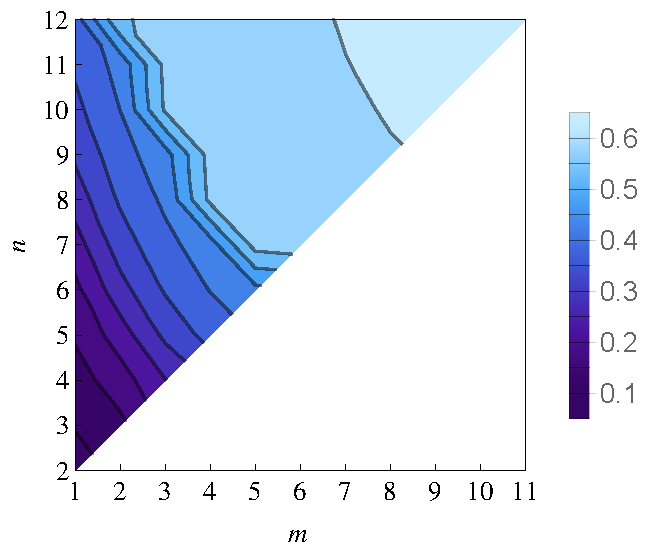
\includegraphics[width=.8\textwidth]{gregory-newton/N14.pdf}
    \caption{Relation of LJ exponents m and n to the difference of largest and
    smallest \ac{COS} distances.  A value of zero would imply that all
    surrounding spheres are touching the center sphere.}
    \label{fig:gregorynewton-N14}
\end{figure}

The results for all positive integer combinations of $m\leq11$ and $n\leq12$
with $m<n$ are depicted in figure~\ref{fig:gregorynewton-N14}. Even for the
combination of smallest exponents (1,2)-\ac{LJ} it is clear that the \ac{COS}
distances vary from sphere to sphere. For this potential the largest \ac{COS}
distance is $r_\text{max}=0.882$, while the shortest one is
$r_\text{min}=0.804$. While the longest distance only shows up once, the
shortest distance appears twice. All other 10 distances fall in the range
between $r = 0.845$ and $r = 0.861$. The $r_\text{max} /r_\text{min}$ ratio is
$1.097$ and much shorter compared to $r_\text{max} /r_\text{min}= \sqrt{2}$ for
the closed packed lattice, or the shortest distance possible for the \ac{SHS}
system which is $r_{14}^\text{GN} = 1.347$ (see discussion below). Hence the
13th sphere ``almost'' touches the center sphere.

Note that all \ac{COS} distances for the $N=14$ (1,2)-\ac{LJ} cluster are
significantly shorter than $r=1$, due to the $N(N-1)/2$ attractive two-body
interactions and the softness of the potential.  For infinite (e.g.
body-centered cubic or close-packed) lattices of particles interacting via
$V^\mathrm{LJ}_{mn}(r)$ with $n> m >3$, one can prove
\autocite{schwerdtfeger_extension_2006} that the nearest neighbor distance is
%
\begin{equation}
    r_\mathrm{NN}(m,n)=\left( L_n L_m^{-1}\right)^\frac{1}{n-m}. %{\color{red} < 1.}
    \label{eqn:lattice}
\end{equation}%
%
Here $L_n$ is the Lennard-Jones-Ingham lattice coefficient for a specific
lattice determined from 3D lattice sums.  Since $L_n<L_m$ for $n>m$, we see
that $r_\mathrm{NN}<1$, and $\lim\limits_{m,n\rightarrow
\infty}r_\mathrm{NN}(m,n)=1$.  The shortest distances found in (6,12)-\ac{LJ}
clusters $r_\text{min}(N)$ are: $r_\text{min}(8)=0.986767$,
$r_\text{min}(9)=0.964404$, $r_\text{min}(10)=0.964382$,
$r_\text{min}(11)=0.956345$, $r_\text{min}(12)=0.947842$, and
$r_\text{min}(13)=0.952179$.  Surprisingly, $r_\text{min}(12)$ is smaller than
$r_\mathrm{NN}(6,12)$ for typical crystalline lattices; $r_\mathrm{NN}(6,12)$
values are $0.95066$, $0.95186$ and $0.97123$ for simple cubic, body-centered
cubic and close-packed lattices, respectively.  This result shows that stable
clusters do not necessarily have longer bonds compared to the solid state,
where we expect a maximum in interaction energy per atom.


\section{The Smallest Gregory-Newton Clusters}
\label{sec:themsmallestgregorynewtonclusters}

Ref.~\cite{holmes-cerfon_enumerating_2016} contains a putatively complete set
of hard-sphere clusters with $N=13$ and $N=14$.  We find a surprisingly large
number ($737$) of nonisomorphic $N = 13$ \ac{GN}-\ac{SHS} structures ($\{724,10,1,2\}$
for $N_c=\{33,34,35,36\}$), that all optimise to the ideal icosahedral
arrangement ($I_h$ symmetry) if a $(6,12)$-\ac{LJ} potential is applied.

\section{Adding a 14th Sphere}
\label{sec:addinga14thsphere}


Most of these $N=14$ clusters are minimally rigid ($N_c=3N-6=36$), while only a
few are hyperstatic ($N_c > 3N-6$) and none are hypostatic ($N_c < 3N-6$).
There are $\{14369,144,8,6,2\}$ such clusters with $N_c=\{36,37,38,39,40\}$ and
$N=14$.  The clusters with $N_c=40$ are hcp and fcc core-shell structures
capped at a square face; these arrangements maximise $N_c$. Most of the
clusters with $N_c=\{38,39\}$ are deformed versions of the elongated pentagonal
bipyramid mentioned above, indicating that this arrangement is a favoured route
to these intermediate-energy structures.  However, $N_c=39$ also contains hcp
and fcc structures capped at a triangular face.  The first example of a cluster
derived from a perfect icosahedral symmetry shows up at lower value $N_c=37$
(!).  Representative examples for clusters with high contact numbers are
depicted in Figure~\ref{fig:N14}.  

\begin{figure}
    \centering
    \subfloat[$r_{14}^\text{GN}=1.34715$, $N_c=39$\label{subfig:short-greg-newton}]{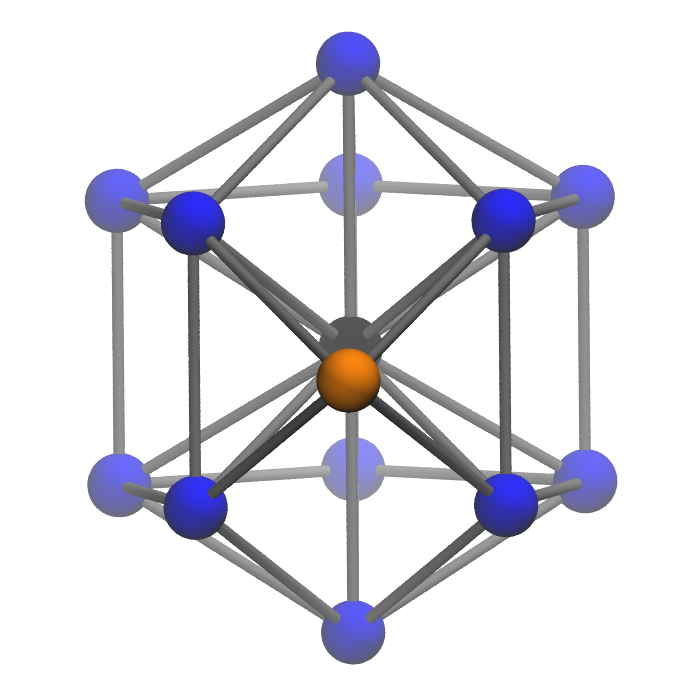
\includegraphics[width=0.4\textwidth]{gregory-newton/short.png}}
    \subfloat[$r_{14}^\text{GN}=1.37515$, $N_c=36$\label{subfig:2ndshort-greg-newton}]{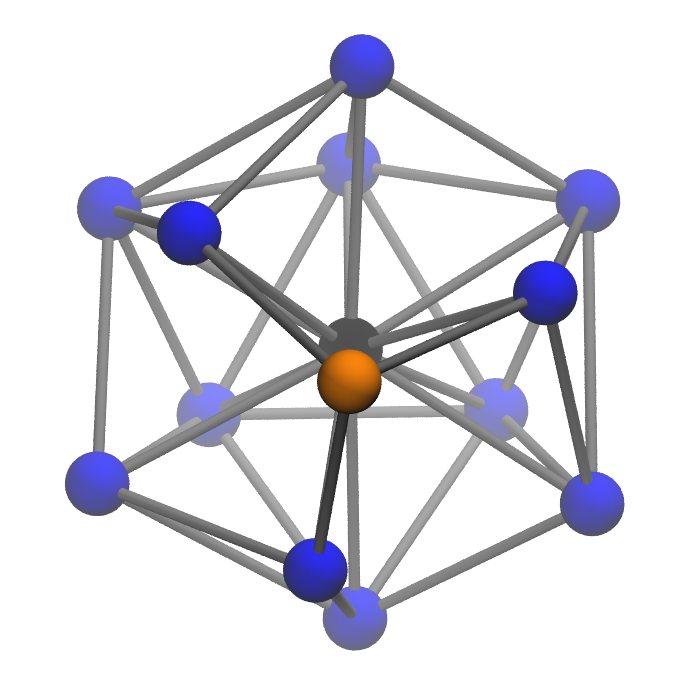
\includegraphics[width=0.4\textwidth]{gregory-newton/2ndshort.png}}\\
    \subfloat[$r_{14}^\text{GN}=\sqrt{2}$, $N_c=40$\label{subfig:sqrt2-greg-newton}]{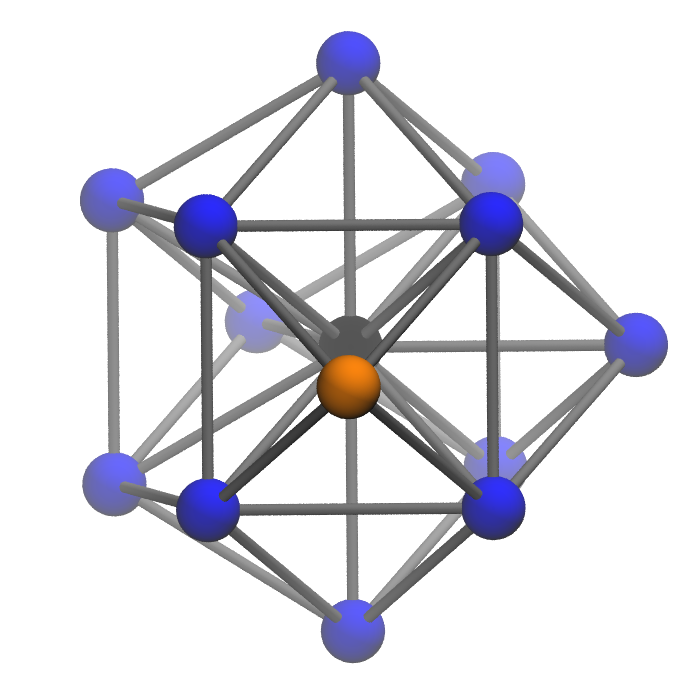
\includegraphics[width=0.4\textwidth]{gregory-newton/sqrt2.png}}
    \subfloat[$r_{14}^\text{GN}=\sqrt{\frac{8}{3}}$, $N_c=39$\label{subfig:sqrt83-greg-newton}]{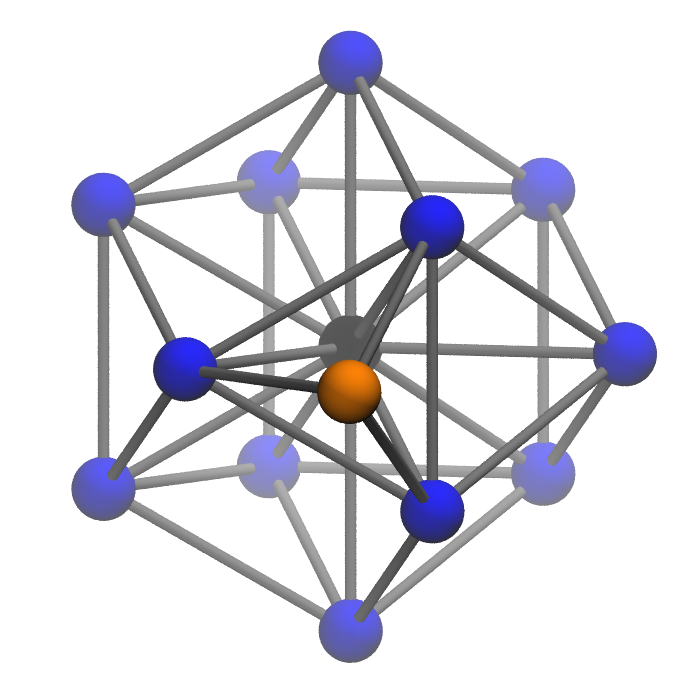
\includegraphics[width=0.4\textwidth]{gregory-newton/sqrt83.png}}\\
    \caption{Graphical representations of SHS packings with $N=14$, where a
center sphere is maximally contacting. The orange sphere in each cluster is the
14th outer sphere, not able to touch the center sphere (in black).  (a)
distorted elongated pentagonal bipyramid (Johnson solid); (b) distorted
icosahedron; (c) hcp capped on a square; (d) hcp capped on a triangle.}
    \label{fig:N14}
\end{figure}

\begin{figure}
    \centering
    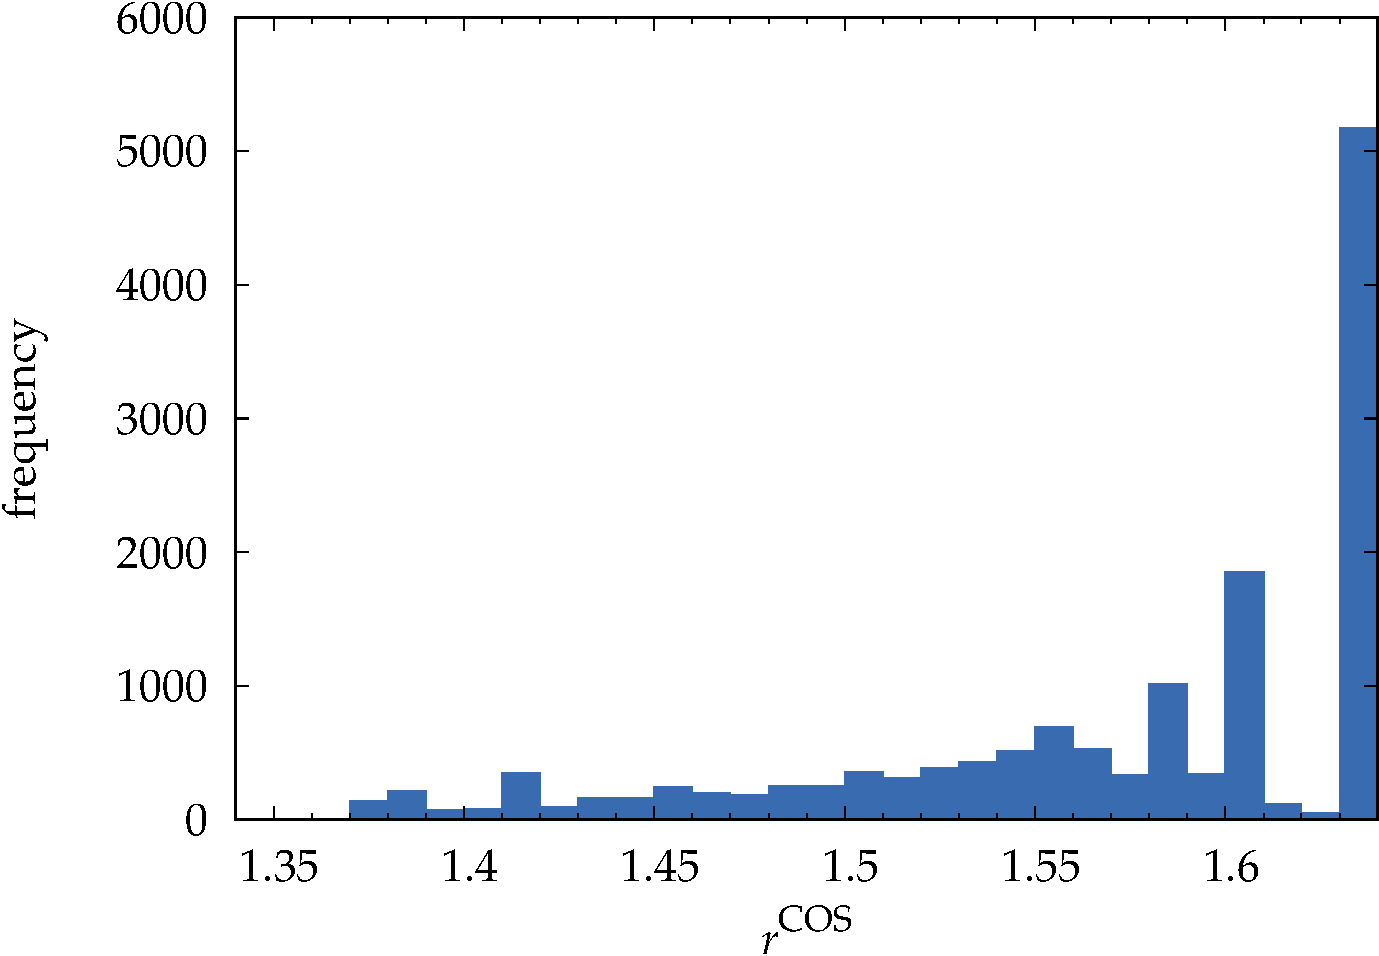
\includegraphics[width=0.8\textwidth]{gregory-newton/greg-newton.pdf}
    \caption{Frequency of distances from the cluster center to the most distant
    sphere for all Gregory-Newton-like clusters contained in the structures
    from Ref.~\cite{holmes-cerfon_enumerating_2016}. The width of the bars is $0.01$.}
    \label{fig:greg-newton}
\end{figure}


Surprisingly, the $N = 14$ cluster with the closest central-to-outer sphere
(COS) distance $r_\text{min}^\text{COS}$ was not known. Here we close this gap by
determining the COS distance for all Gregory-Newton type clusters.  We find one
single cluster with $r_\text{min}^\text{COS}=1.3471506281091$.  Its structure
(Fig.\ \ref{subfig:short-greg-newton}) is similar to the elongated pentagonal bipyramid (a
Johnson solid) with one of the square faces stretched to form a regular
rectangle.  The 14th sphere caps this deformed face, becoming the vertex of a
deformed octahedron and allowing the outer sphere to get closer to the central
sphere.  The next-smallest-$r^\text{COS}$ cluster ($r^\text{COS} = 1.37515$) is
shown in Fig.~\ref{subfig:2ndshort-greg-newton}.  It does not belong to the
category of the clusters derived from the elongated pentagonal bipyramid, but
instead can be described as being icosahedral-like.  The short distance is
achieved by attaching the 14th sphere to 3 spheres that do not form a face of
the cluster (because they are separated by a distance larger than $1$.)


As shown in Figure \ref{fig:greg-newton}, the distribution of $r^\text{COS}$
values for the full set of \ac{GN} clusters is shown in Figure
\ref{fig:greg-newton}.  Motifs with larger $r^\text{COS}$ are far more
prevalent.  For example, the peak at $r^\text{COS} = 1.41$ corresponds to
structures where the 14th sphere is touching 4 other spheres that are part of a
tetragonal pyramid, therefore forming a regular octahedron with a tip-to-tip
distance of $\sqrt{2}$ (Fig.~\ref{subfig:sqrt2-greg-newton}).  The maximum
$r^\text{COS}$ value ($1.63$) corresponds to capping triangular faces, so that
the most distant sphere is part of a regular trigonal bipyramid with a height
of $\sqrt{8/3}$ (Fig.~\ref{subfig:sqrt83-greg-newton}).  The structures in the
bars at $1.60,1.58$ and $1.55$ are derived from the regular trigonal bipyramid
and result from breaking its axial bonds.  In these structures, the more bonds
are broken, or the further the axial spheres are separated, the shorter the
center-to-outer sphere distance becomes.
